\chapter{Einleitung}

Softwarequalitätsmanagement (SQM) ist ein entscheidender Aspekt bei der Entwicklung und Implementierung von Softwarelösungen, 
um sicherzustellen, dass sie effizient, sicher und zuverlässig sind. In dieser Hausarbeit werden wir uns mit dem Vorgehen 
hinsichtlich SQM auseinandersetzen und Optimierungen entwerfen, indem wir ein praktisches Fallbeispiel untersuchen. 
Unser Anwendungsbeispiel ist die Integration einer Recommendation Engine (RE) in eine Lernplattform mit Gamification 
auf dem Hyperscaler Amazon Web Services (AWS). Dieses Beispiel dient dazu, sowohl theoretisches Wissen als auch praktische 
Anwendungsfähigkeiten in Bezug auf SQM nachzuweisen.

Bei meiner Firma, der SAP, gibt es intern eine Lernplattform die Gamification nutzt, um SAP-interne Prozesse 
spielerisch den Kollegen zu vermitteln. Diese Plattform heißt \textit{Digital Heroes}. 
Bisher können die Kollegen die Lernplattform nach konkreten Inhalten durchsuchen. 
Außerdem können die Moderatoren bestimmte Inhalte auf der Startseite featuren. Es gibt jedoch keine 
personalisierten Empfehlungen von Lerninhalten für die Nutzer der Plattform. 
Durch das Einführen einer in-house RE soll sich das nun ändern und damit den Prozess für Nutzer an neue Inhalte 
zu gelangen verbessern.  \\
Das Problem beim Integrieren der RE ist allerdings, dass die bisherige Software dafür angepasst 
und vorbereitet werden muss. Insbesondere arbeitet die RE auf stark-assoziierten Daten, 
was viele sehr aufwendige Joins in der derzeitig genutzten relationalen Datenbank nötig macht, 
was sehr ressourcenintensiv ist.  
Ziel des hier genutzten Anwendungsbeispiels ist es also die RE in die bestehende Software so zu integrieren, 
dass andere Systemteile nicht beeinträchtigt werden. 

Um dieses Ziel zu erreichen, soll das erworbene Wissen aus der Softwarequalität-Vorlesung genutzt werden, 
um das Problem kritisch zu analysieren und zu optimieren. 
Dafür wird zunächst die Ausgangssituation des aktuellen Prozesses untersucht, 
daraufhin wird betrachtet, warum die RE eingeführt wird und warum das bestimmte Anpassungen an der 
bestehenden Software nötig macht. Darauf aufbauend wird beschrieben, wie dadurch der bestehende 
Prozess verbessert werden kann. Weiter wird analysiert, welche Optimierungsmöglichkeiten aus der Sicht 
der SQM es hierfür gibt. Anschließend wird betrachtet, wie der Prozess nach der Optimierung aussieht. 
Schließlich werden in einer Zusammenfassung die grundlegenden Erkenntnisse der Arbeit nochmals bündig dargelegt.

\chapter{Derzeitiger Prozess}

Die gamifizierte Lernplattform namens Digital-Heroes (DH) kann derzeit nach Lerninhalten durchsucht werden 
und es werden \textit{Featured Missions} angezeigt.
Bei dem Durchsuchen nach Lerninhalten kann derzeit eine Volltextsuche verwendet werden. 
Es kann zudem nach groben Kategorien geordnet werden. 
Die Featured Missions, die in \autoref{fig:dh-website} abgebildet sind, 
werden durch das Moderatorenteam ausgewählt -- es steht kein automatischer 
Algorithmus dahinter.

\begin{figure}
	\centering
	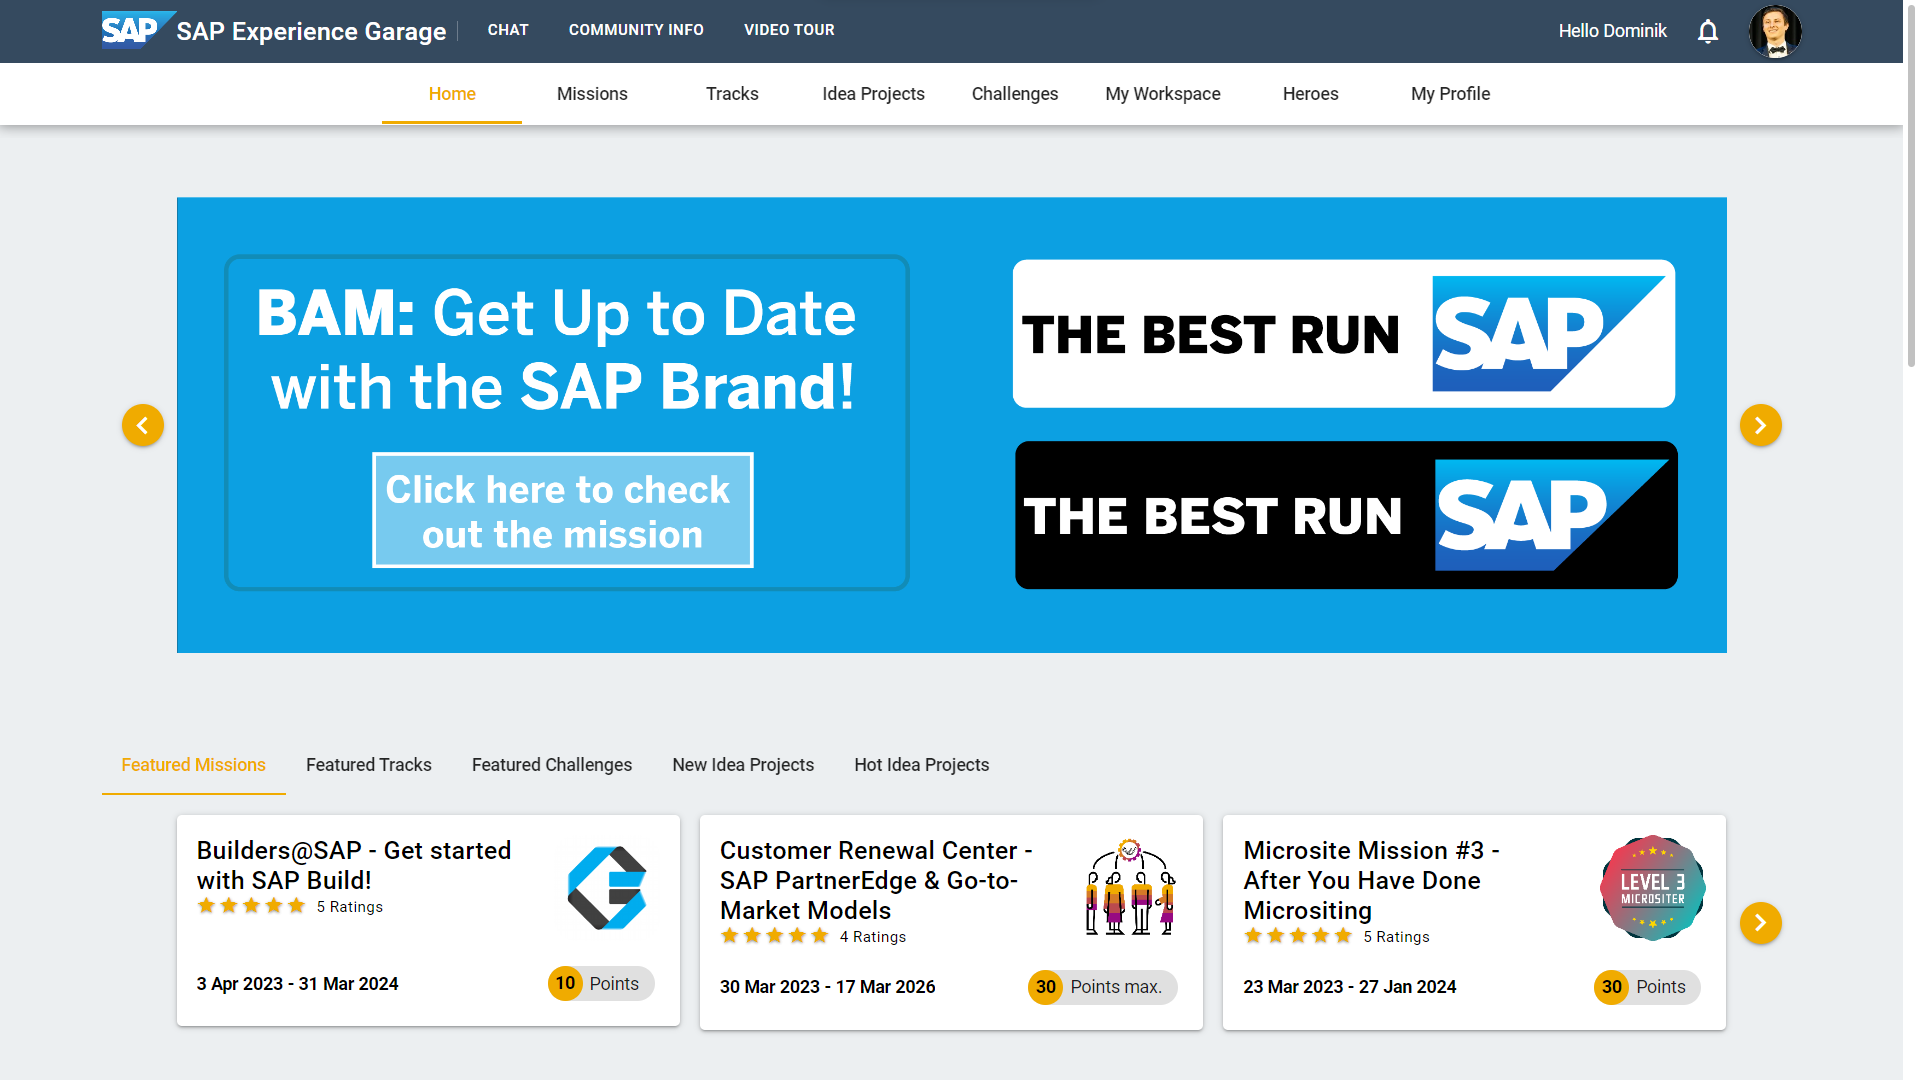
\includegraphics[width=1.\textwidth]{Bilder/dh-website.png} 
	\caption{Die Abbildung zeigt die Landing-Page der Digital-Heroes-Lernplattform. 
    Insbesondere lässt sich der Tab der \textit{Featured Missions} erkennen.}
	\label{fig:dh-website}
\end{figure} 
